\section{Gebruikers Beschrijving}

\subsection{Belanghebbenden}
In deze sectie van het SRD worden de belanghebbende van de opdracht geïdentificeerd. Er zal ook worden beschreven wat de behoeften zijn van de belanghebbenden, die uiteindelijk zullen worden overwogen in het ontwerpproces.

\textbf{Belanghebbenden:}

\begin{itemize}
	\item \textbf{Customer Service (Hoofdgebruiker van de testkast)}
	\begin{itemize}
		\item De customer serviceafdeling zal de testkast gaan gebruiken om teruggestuurde spindels te testen en te analyseren. De behoeften van deze afdeling zullen zijn:
		\begin{enumerate}
			\item Een gebruiksvriendelijke interface om verschillende spindels te testen op de testkast.
			
			\item De testresultaten moeten betrouwbaar zijn en reproduceerbaar.
			
			\item Log bestanden en testrapporten om analyses uit te voeren.
			
			\item Test criteria waar de motoren aan moeten voldoen zodat ze als goed of slecht kunnen worden bestempeld.
			
			\item Meerdere soorten motoren moeten werken op de testkast.
			
			\item Documentatie om de kast te bedienen.
		\end{enumerate}
	\end{itemize}
	
	\item \textbf{Operators (Dagelijkse gebruikers van de testkast)}
	\begin{itemize}
		\item De operators van de testkast zijn de mensen die de kast daadwerkelijk gaan gebruiken. Hun behoeften kunnen zijn:
		\begin{enumerate}
			\item Een gemakkelijke manier om de testparameters voor een specifieke spindel te selecteren.
			
			\item Een veilig systeem wat de risico’s minimaliseert tijdens het testen van de spindels.
			
			\item Een testproces wat niet te veel tijd kost.
			
			\item Duidelijke feedback van de testkast als eventuele problemen zich voor doen. (Foutmeldingen of waarschuwingen)
			
			\item Eventueel vertaalde tekst op het scherm in andere talen.
		\end{enumerate}
	\end{itemize}
	
	\item \textbf{Onderhoudsdienst}
	\begin{itemize}
		\item De onderhoudsdienst is verantwoordelijk voor het onderhoud van de testkast en eventuele uitbreiding van de kast. De behoeften van deze groep is:
		\begin{enumerate}
			\item Goede documentatie van de code.
			
			\item Inzicht in de parameters en instellingen van de testkast.
			
			\item Goed documentatie van de hardware.
		\end{enumerate}
	\end{itemize}
	
	\item \textbf{R\&D Engineering Team}
	\begin{itemize}
		\item Wanneer Voortman besluit nieuwe machines te ontwikkelen met mogelijk nieuwe type spindels kan de testkast ook nuttig zijn voor de R\&D. Zij zouden de volgende dingen willen:
		\begin{enumerate}
			\item Makkelijk nieuwe testscenario’s kunnen instellen voor de nieuwe motoren.
			
			\item Overzicht over de prestaties van de spindel.
		\end{enumerate}
	\end{itemize}
	
	\item \textbf{Klanten van Voortman}
	\begin{itemize}
		\item Klanten die de gereviseerde motor uiteindelijk kopen kunnen ook baat hebben bij de testkast zij zouden de volgende dingen willen hebben:
		\begin{enumerate}
			\item Een testrapport waarin te zien is dat de gekochte gereviseerde spindel correct werkt naar behoren.
		\end{enumerate}
	\end{itemize}
\end{itemize}

\newpage

\subsection{Gebruikersscenario(s)}

In deze sectie worden alle verschillende gebruikersscenario’s geschetst om de interactie die de gebruiker heeft met het systeem te visualiseren. De volgende stappen moeten doorlopen worden om de spindel juist aan te sluiten en te testen op de testkast.

\begin{figure}[H]
	\centering
	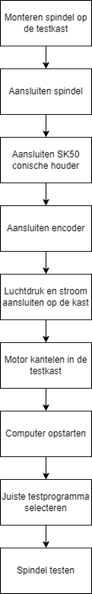
\includegraphics[width=0.18\linewidth]{Gebruikersscenario}
	\label{fig:Gebruikersscenario}
	\caption{Gebruikersscenario spindel bedienen}
\end{figure}